\documentclass[a4paper, 11pt]{article}
\usepackage[utf8]{inputenc}   % Pour lire les fichiers UTF-8
\usepackage[T1]{fontenc}      % Pour une meilleure gestion des caractères accentués
\usepackage{textcomp}         % Pour quelques symboles supplémentaires
\usepackage{lmodern}          % Police compatible avec T1
\usepackage[english,french]{babel} 
\usepackage{graphicx} % Pour les images
\def\@captype{figure}
\usepackage{float}
\usepackage{multicol} % Pour faire des multi colonnes
\usepackage[export]{adjustbox} % Pour la clé 'valign'  (aligner verticalement)
\usepackage[colorlinks=true,linkcolor=black]{hyperref} % Pour qu'il y est des liens sur la table des matières
\usepackage{caption} % Utiliser plus de fonction sur caption (caption* pour ne pas afficher FIGURE-1)
\usepackage{lipsum} % Pour générer du texte pour voir comment ca rend
\usepackage{ragged2e} % Pour justifier le texte
\usepackage{ulem}
\usepackage[margin=3.2cm]{geometry}
\usepackage{forest}
\usepackage{listings}
\usepackage{xcolor}
\usepackage{amsmath}
\usepackage{amssymb}
\usepackage{fancybox}
\usepackage{fancyhdr}
\usepackage[none]{hyphenat}
\emergencystretch=3em
\usepackage{graphicx}
\usepackage{adjustbox}
\usepackage{float}
\usepackage[section]{placeins} % OK


\usepackage{csquotes}


% Configuration de fancyhdr
\pagestyle{fancy}
\fancyhf{} % Efface tous les en-tètes et pieds de page précédents
\fancyhead[C]{Rapport de Projet} % Texte centré en haut de la page
\fancyfoot[L]{2025} % Texte en bas à  gauche du pied de page
\fancyfoot[C]{COUTANT, LITAMPHA, PETER} % Texte au centre du pied de page
\fancyfoot[R]{\thepage} % Numéro de page en bas à  droite du pied de page

\renewcommand{\headrulewidth}{0.4pt} % à‰paisseur de la ligne de séparation de l'en-tète
\renewcommand{\footrulewidth}{0.4pt} % à‰paisseur de la ligne de séparation du pied depage
\setlength{\headheight}{13.59999pt}
% Appliquer le style d'en-tète fancy aux pages de début de chapitre

\fancypagestyle{plain}{
  \fancyhf{} % Effacer tous
  \fancyhead[C]{Rapport de Projet} % Texte centré en haut de la page
  \fancyfoot[L]{L3 Informatique} % Texte en bas à  gauche du pied de page
  \fancyfoot[C]{COUTANT, LITAMPHA, PETER} % Texte au centre du pied de page
  \fancyfoot[R]{\thepage} % Numéro de page en bas à  droite du pied de page
  \renewcommand{\headrulewidth}{0.4pt} % à‰paisseur de la ligne de séparation de l'en-tète
  \renewcommand{\footrulewidth}{0.4pt} % à‰paisseur de la ligne de séparation du pied de page
}




\begin{document}

% Page de titre

% Page de titre
\begin{titlepage}
    \centering
    \vspace{3cm}
    \includegraphics[width=0.4\textwidth]{images/logo_univ.jpg}\hfill
    \includegraphics[width=0.5\textwidth]{images/logo_ufrst.png}\\
    \vspace{1.5cm}
    {\huge \textbf{Université Marie \& Louis Pasteur\\ UFR Sciences et Techniques}\par}
    \vspace{0.5cm}


    \shadowbox{\parbox{0.9\linewidth}{\centering \huge \textbf{Projet L3 : Pacman en réseau}}}\\
    \vspace{1cm}
    {\Large \textbf{Rapport de Projet} \\ Licence CMI Informatique - 3ème année \\ 2025-2026\par}
    \vspace{0.5cm}

    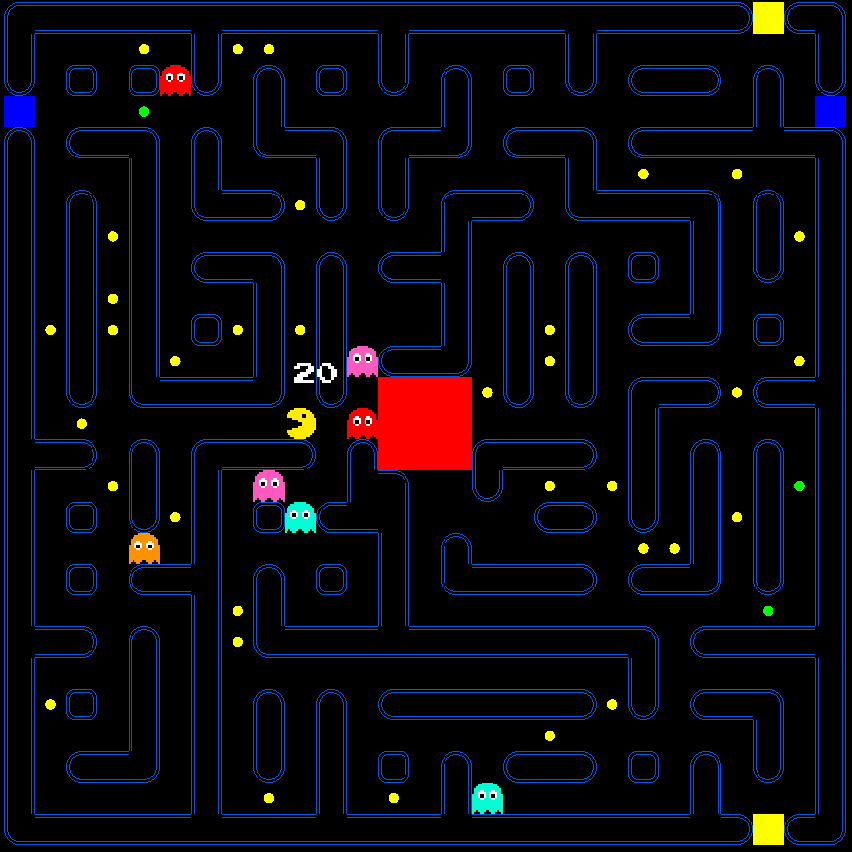
\includegraphics[width=0.7\textwidth]{images/entete.png}\\
    \vspace{0.5cm}

    {\LARGE \textbf{Thomas COUTANT}\\ \textbf{Benoît LITAMPHA}\\ \textbf{Auriane PETER}\par}
    \vspace{1cm}
    {\large \textbf{Encadrant : Julien BERNARD} }\\

    
\end{titlepage}


    


\section*{Remerciements}
\addcontentsline{toc}{section}{Remerciements}
\newpage


\tableofcontents
\listoffigures
\newpage



\section*{Introduction}
\addcontentsline{toc}{section}{Introduction}



\vfill


\section{Présentation du projet}


\subsection{Présentation générale du jeu \texttt{Pac-Man}}

Le jeu \texttt{Pac-Man}, apparu au début des années 1980, est un jeu d’arcade dans lequel le joueur contrôle un personnage évoluant dans un labyrinthe. L’objectif principal est de parcourir l’ensemble du labyrinthe afin de consommer toutes les \texttt{pac-gommes} qui s’y trouvent, tout en évitant d’entrer en contact avec des fantômes. Ces derniers constituent les adversaires du joueur et cherchent à bloquer ou intercepter ses déplacements. Certaines \texttt{pac-gommes} spéciales permettent temporairement à \texttt{Pac-Man} d’inverser les rôles en devenant capable de manger les fantômes, ajoutant ainsi une dimension stratégique au gameplay.

\begin{figure}[H]
    \centering
    \includegraphics[width=0.8\textwidth]{images/pac_man_original.png}
    \caption{PacMan : le jeu original}
\end{figure}


Dans le cadre de ce projet, le jeu a été adapté pour le multijoueur. Une partie oppose un joueur \texttt{Pac-Man} à plusieurs joueurs fantômes. Lorsque le nombre de joueurs est insuffisant, certains fantômes sont controlés par des intelligences artificielles afin de ne pas déséquilibrer la partie.

Le choix de \texttt{Pac-Man} comme sujet pour une version en réseau est stratégique car ses règles simples et très connues, ce qui permet une facilité d'implémentation par rapport a d'autre jeux. De plus, le gameplay se prête à une séparation des rôles entre plusieurs joueurs.

\subsection{Contexte académique}

Ce projet a été réalisé dans le cadre du semestre six de la licence informatique de l’Université Marie \& Louis Pasteur. Il s’inscrit dans un enseignement visant à mettre en pratique nos connaissances à travers la réalisation d’un gros projet à plusieurs.

Le travail a été mené en groupe de trois étudiants de mi-octobre à la fin du mois de mars, sous l’encadrement de Julien Bernard, maître de conférences à l’Université Marie \& Louis Pasteur. Le projet porte sur le développement d’un jeu vidéo en réseau.

Les objectifs de ce projet sont de consolider nos compétences en programmation C++, approfondir la découverte du développement de jeux vidéo, ainsi qu’à mettre en place une architecture réseau client–serveur. Le projet permet également de développer des compétences telles que le travail en équipe et la gestion d’un projet informatique sur une longue période.


\subsection{Objectifs généraux du projet}

Les objectifs du projet peuvent être divisés en deux catégories : 
\begin{itemize}
    \item les objectifs fonctionnels, liés à l’expérience de jeu
    \item les objectifs techniques, liés à la conception et à l’implémentation du système\\
\end{itemize}


Du point de vue fonctionnel, l’objectif était de concevoir un jeu Pac-Man jouable en réseau qui permet à plusieurs joueurs de participer à une même partie.

Sur le plan technique, le projet visait à mettre en place une architecture réseau client–serveur. Le serveur devait être capable de gérer les connexions des joueurs, la création et la gestion des parties, ainsi que l’échange des données nécessaires au jeu.

\newpage


\section{Définition du sujet et problématique}

\subsection{Problématique du jeu en réseau}

La conception d’un jeu multijoueur en temps réel implique plusieurs contraintes. La difficultée majeur concerne la synchronisation des états du jeu entre les clients. Chaque joueur doit avoir une vision cohérente de l’ensemble de la partie (les positions de Pac-Man, des fantômes et l’état des pac-gommes, ect). Pour garantir cette cohérence, nous avons opté pour un serveur autoritaire : toutes les décisions sont validées côté serveur, qui diffuse ensuite les informations à tous les clients. Qui, de leur côté, envoient uniquement leurs intentions de déplacement, qui sont ensuite traitées et synchronisées par le serveur. Les données transitent via des buffers et des files avant d’être appliquées. Cela permet un traitement ordonné des événements du jeu.

\subsection{Choix techniques}

Le projet devait être développé en C++ en utilisant la bibliothèque \textit{Gamedev Framework} (gf), qui est adaptée au développement de jeux vidéo et est compatible avec l’architecture réseau. La communication réseau repose sur le protocole TCP, assurant la sûreté des échanges entre le serveur et les clients. Les messages sont sérialisés afin de structurer les informations transmises.

Nous avons par contre choisi de concevoir le serveur selon un modèle multithread avec une chaine de responsabilitée pour gérer les packets, reflétant la logique de fonctionnement du jeu : un thread\footnote{Un thread (fil d’exécution) est une unité d’exécution légère au sein d’un processus. Dans une architecture client-serveur, il permet par exemple de gérer plusieurs connexions ou tâches simultanément (réception réseau, logique de jeu, envoi des mises à jour) tout en partageant la même mémoire.} principal gère le serveur et le lobby, tandis que d’autres threads s’occupent des rooms, de la boucle de jeu, des fantômes contrôlés par l’IA et de la communication avec les clients. Cette architecture permet de traiter simultanément plusieurs interactions des joueurs et d’assurer une exécution fluide et cohérente des parties.

\begin{figure}[H]
    \centering
    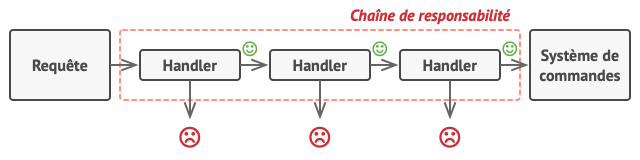
\includegraphics[width=1\textwidth]{images/chaine_responsabilité.png}
    \caption{Exemple de Chaine de responsabilité}
\end{figure}

\subsection{Répartition des rôles}

La réalisation de ce projet a été organisée de manière collaborative entre les trois membres du groupe. 

Thomas Coutant a principalement travaillé sur le développement du serveur, ainsi que sur la conception de la logique du jeu. Il a également développé un prototype minimal de démarrage, permettant de tester la communication client–serveur avec un simple cube représentant un joueur en mouvement.

Auriane Peter s’est concentrée sur le développement du client, en implémentant l’interface et la gestion des interactions côté joueur.

Benoît Litampha a assuré la communication entre le serveur et le client, participant également à certaines tâches sur le serveur et le client lorsque nécessaire. 

Cette répartition a permis une progression simultanée sur plusieurs fronts du projet, tout en gardant une cohérence globale de l’application.
\newpage

%\section{L'Organisation du stage}


\section{Architecture et conception}

\subsection{conception du jeu}

Les règles du jeu ont été définies afin de mettre en place un équilibre entre tension et stratégie.
Chaque camp dispose d’objectifs et contraintes différents, créant une structure de compétition.

\subsubsection{Conditions de victoire}

Pac-Man gagne la partie s’il parvient à manger tout les pac-gommes du plateau ou s’il survit jusqu’à la fin du timer. 
Les fantômes, eux, gagnent en épuisant toutes les vies de Pac-Man avant la fin du temps imparti.

Ce double système de victoire met une pression permanente : Pac-Man doit optimiser ses déplacements, tandis que les fantômes doivent coordonner leurs actions pour limiter ses déplacements.

\subsubsection{Pac-gommes spéciales}

Certaines pac-gommes déclenchent un mode temporaire appelé « chasseur ».
Durant cette période, Pac-Man devient capable de manger les fantômes.
Cet état est limité dans le temps par un timer.
Les fantômes éliminés réapparaissent mais ont aussi des vies, maintenant ainsi l’équilibre de jeu car les pac-gommes spéciales sont peu nombreuse.

Ce mécanisme introduit un changement brutale du gameplay, les chasseurs deviennent les chassés et inversement.

\subsubsection{Asymétrie de vision}

Le système repose également sur une différence de vision.
Pac-Man a une vue globale du plateau, tandis que les fantômes ne voient uniquement environnement limités, ils ne peuvent voir qu'a une certaines distance d'eux même, la vison des fantomes n'est pas partagée entre eux.

\subsubsection{Cohérence du système}

La combinaison de ces règles avec la génération procédurale du plateau et l’architecture hybride de l’intelligence artificielle et des joueurs, produit un gameplay varié et imprévisible.
Les interactions entre le timer, le manque de vision et inversement temporaire des rôles permettent de nombreuse stratégies et augmentent la rejouabilité du jeu.



\subsection{Structure du serveur}

\subsubsection{Architecture multithread}

Le serveur repose sur une architecture multithread\footnote{Un programme multithread exécute plusieurs fils d'exécution (threads) en parallèle au sein d’un même processus.} conçue pour supporter plusieurs connexions simultanées sans dégradation des performances. 
La couche réseau est strictement séparée de la logique de jeu afin d’éviter qu’une opération bloquante, attente de paquet\footnote{Un paquet réseau est une unité de données formatée et structurée, transmise à travers un réseau. Il contient généralement une en-tête (header) avec des informations de routage et de contrôle, ainsi qu’une charge utile (payload) correspondant aux données transportées.}, latence élevée ou déconnexion, n’impacte l’exécution globale du système.

Un thread est dédié à la réception des paquets réseau. 
Les messages entrants sont insérés dans une file d’attente interne, puis traités de manière synchronisée par la logique centrale du serveur. 
Cette organisation assure une séparation claire entre la  communication et la logique.

La file de messages agit comme un tampon entre le réseau et la boucle de jeu à tick\footnote{Un tick désigne une unité de temps discrète utilisée par le moteur du jeu pour mettre à jour l’état du monde. À chaque tick, le serveur traite les entrées des joueurs, met à jour la logique de jeu (physique, collisions, scores, etc.) puis envoie les nouvelles informations aux clients.} fixe. 
Ainsi, les mises à jour périodiques du monde restent indépendantes des variations de latence ou du débit des clients.

Cette architecture permet l’exécution simultanée de plusieurs parties indépendantes au sein d’un même serveur.

\begin{figure}[H]
    \centering
    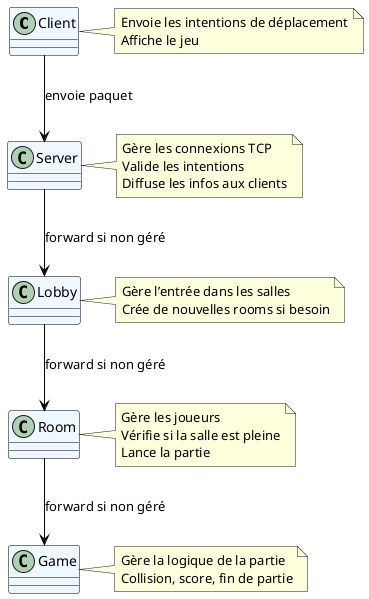
\includegraphics[width=0.6\textwidth]{UML/PacMan_UML_Server_chaine.png}
    \caption{Chaîne de responsabilité côté serveur}
\end{figure}

\subsubsection{Architecture modulaire}

L’architecture du serveur est organisée en plusieurs couches distinctes possédant chacune une responsabilité. 
Cette structuration modulaire garantit lisibilité, extensibilité et maintenabilité.

La couche \textit{Server} assure la gestion des connexions et le routage des messages. 
Le \textit{Lobby} centralise l’organisation des joueurs et la création des parties. 
Chaque partie est enfermé dans une entité \textit{Room}, responsable de son état propre et de ses joueurs. 
Enfin, la logique complète du jeu est contenue dans la classe \textit{Game}, indépendante des mécanismes réseau.

L’architecture suit ainsi une chaîne de responsabilité hiérarchique :

\begin{center}
Client $\rightarrow$ Server $\rightarrow$ Lobby $\rightarrow$ Room $\rightarrow$ Game
\end{center}

Chaque couche délègue les traitements spécialisés au niveau inférieur, ce qui permet d’introduire de nouvelles fonctionnalités sans modifier les composants fondamentaux du système.


\begin{figure}[H]
    \centering
    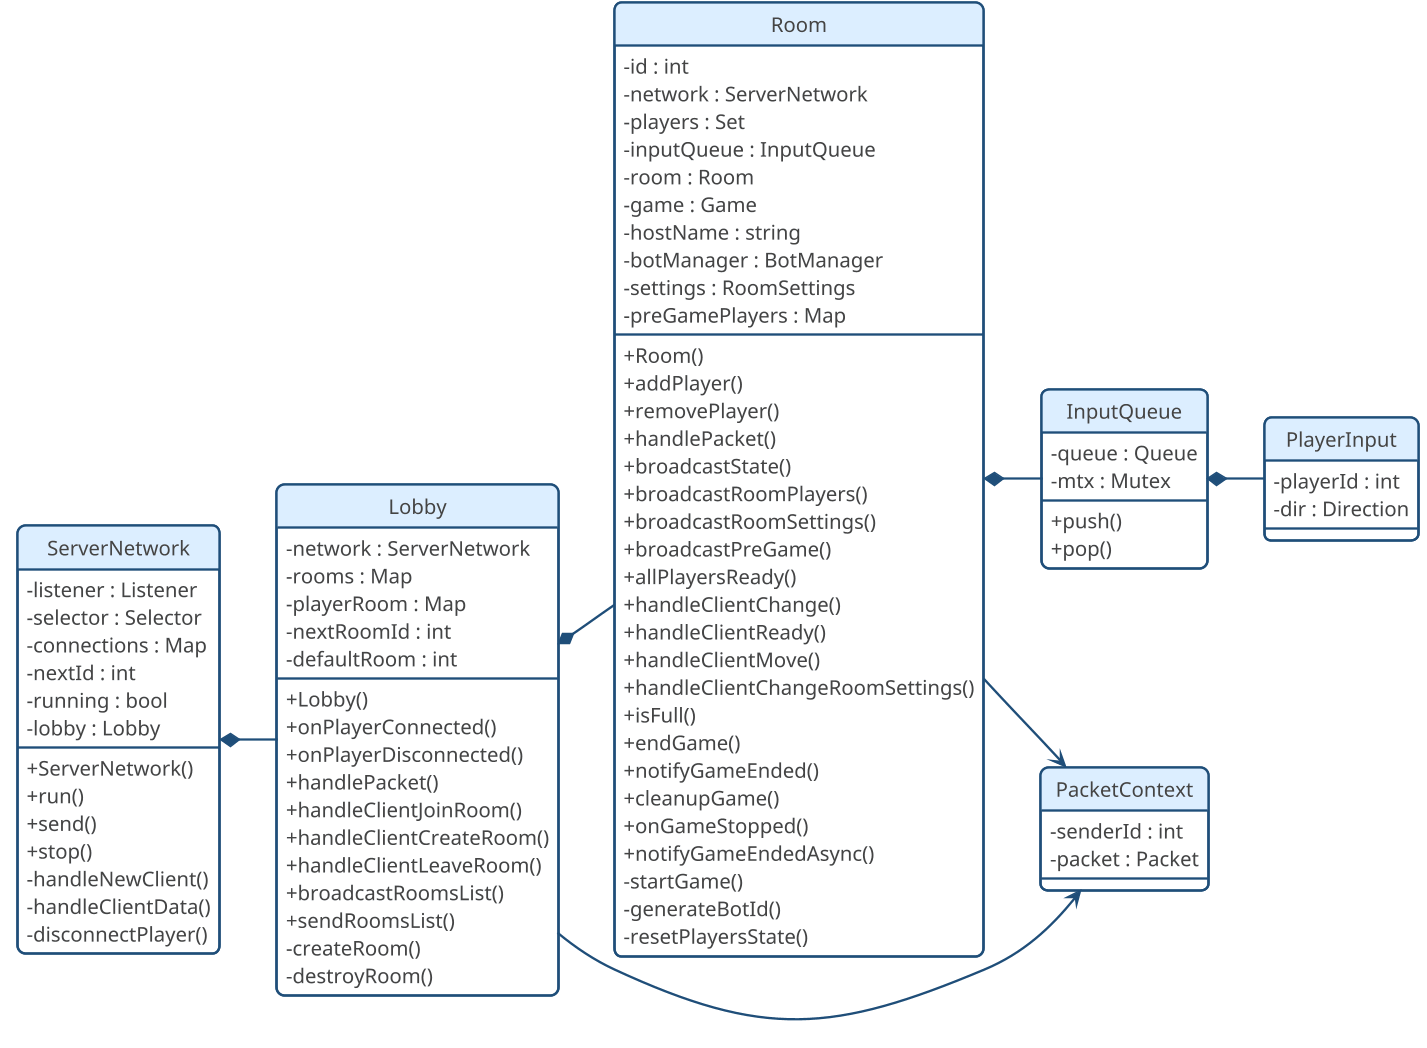
\includegraphics[width=1\textwidth]{UML/PacMan_UML_Server_Reseau.png}
    \caption{Diagrammes de classe de l'architecture réseau}
    \caption*{Vue côté serveur - Gestion des packets, des parties, des salles (sans geter et seter)}

\end{figure}

\subsubsection{Structure du plateau}

Le plateau est modélisé sous forme d’une grille en deux dimensions, composée de cases murales et de cases traversables. 
Cette représentation constitue la base logique du système.

Il sert de référence unique pour la détection des collisions, la mise à jour des déplacements, le placement des éléments interactifs ainsi que pour les algorithmes d’intelligence artificielle. 
La cohérence entre la logique côté serveur et l’affichage côté client offre une synchronisation fiable du jeu.

Le plateau constitue une structure centrale sur laquelle reposent la génération procédurale du labyrinthe et les mécanismes décisionnels des fantômes.

\subsubsection{Boucle de jeu}

La boucle de jeu constitue le cœur du serveur et repose sur un modèle à mise à jour périodique, appelé \textit{tick serveur}. 
Contrairement à une architecture purement événementielle, l’état du monde est recalculé à intervalle régulier selon une fréquence fixe. 
Ce fonctionnement garantit un comportement déterministe et centralisé.

À chaque tick, le serveur exécute une séquence d’opérations. 
Les intentions de déplacement reçues des clients sont d’abord traitées, puis les positions des entités sont mises à jour en fonction des règles. 
Les états temporaires sont ensuite décrémentés, le score est ajusté et les conditions de fin de partie sont vérifiées.

Les rôles sont attribués au début de chaque partie : un joueur incarne Pac-Man tandis que les autres incarnent les fantômes. 
Chaque rôle possède des contraintes qui influence les déplacements et les interactions. 
L’ensemble de ces règles est appliqué exclusivement côté serveur, il est le seul qui décide.

Le plateau contient deux types de pac-gommes. 
Les pac-gommes classiques augmentent le score lors de leur consommation, tandis que les pac-gommes spéciales déclenchent un mode temporaire dit « chasseur ». 
Ce mode est géré par un système de minuterie interne décrémenté. 
Lorsque ce compteur atteint zéro, l’état normal est restauré.

Il y a 2 timers, un timer global définissant la durée maximale d’une partie, et un timer local associé aux états temporaires. 
Cette gestion du temps garantit une certaine cohérence entre les événements et permet l'indépendance des événements du jeu.

Les collisions sont évaluées avant chaque chaque mise à jour de position. 
Un déplacement vers une case murale est annulé ou sur une case hut pour \texttt{PacMan}. 
Lors d’une collision entre Pac-Man et un fantôme, l’issue dépend de l’état courant : perte d’une vie en mode normal, perte d’une vie du fantôme en mode chasseur. 
L’intégralité de ces calculs étant effectuée côté serveur, toute tentative de triche ou de désynchronisation est neutralisée.

À la fin de chaque tick, l’état global mis à jour est diffusé à l’ensemble des clients. 
Ces derniers ne réalisent aucun calcul logique : ils se contentent d’afficher l’état reçu. 
Cette architecture s’inscrit dans le modèle de serveur autoritaire défini précédemment.

\subsubsection{Plateau et génération procédurale}

Le plateau repose sur une génération procédurale de labyrinthe fondée sur une variante de l’algorithme de Prim. 
Ce choix permet de produire automatiquement des cartes connexes avec une forte variabilité entre les parties.

La génération débute par un remplissage complet du plateau avec des murs. 
Une case de départ est ensuite sélectionnée et marquée comme traversable. 
Ses murs adjacents sont ajoutés à une liste dite \textit{frontier}. 
À chaque itération, un mur est choisi aléatoirement dans cette liste. 
S’il sépare une case déjà accessible d’une case encore murale, il est supprimé, la nouvelle case devient traversable, et ses propres murs sont ajoutés à la frontier. 
Le processus se poursuit jusqu’à épuisement de cette liste.

Ce mécanisme produit un arbre couvrant avec un labyrinthe connexe sans zones isolées.

\begin{figure}[H]
    \centering
    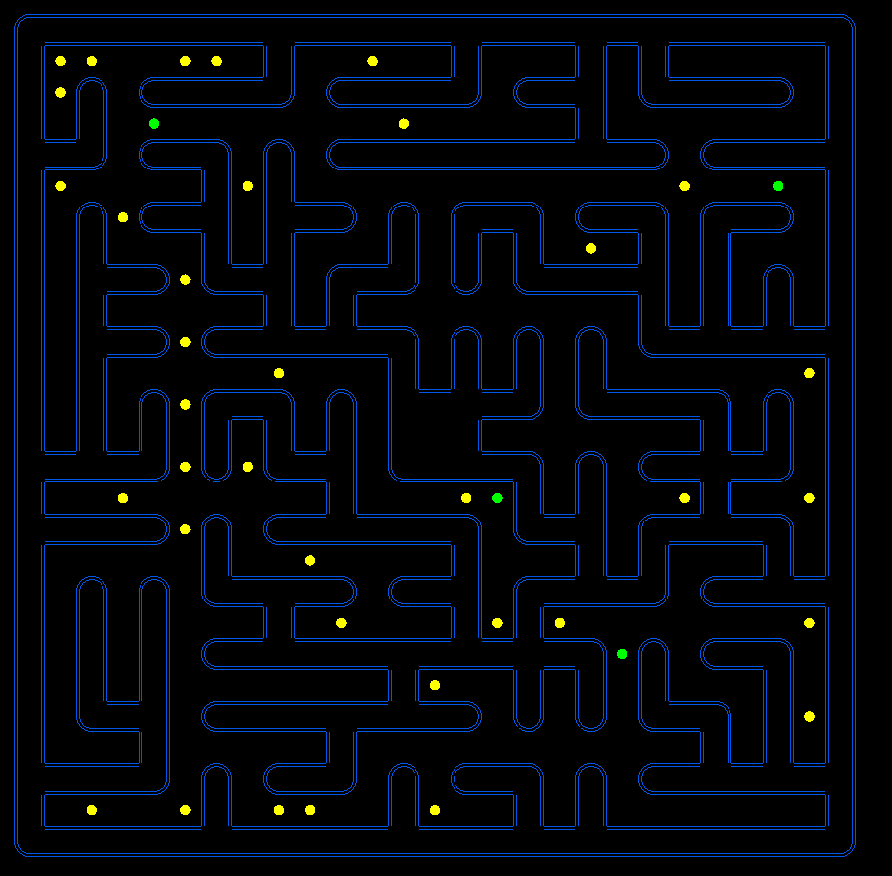
\includegraphics[width=1\textwidth]{images/plateau_42_1.png}
    \caption{Plateau apès l'algorithme de Prim}
\end{figure}

Afin d’adapter cette structure aux contraintes du gameplay, plusieurs transformations supplémentaires sont appliquées.

Une zone centrale fixe de taille $3 \times 3$, appelée « hut », est réservée avant la génération. 
Elle est protégée durant l’exécution de l’algorithme afin de préserver sa structure. 
Une fonction dédiée vérifie ensuite son raccordement au labyrinthe principal par au moins une ouverture.

Les coins du plateau, destinés aux positions initiales des joueurs, sont également vérifiés après la génération. 
Si l’un d’eux se retrouve isolé, une ouverture contrôlée est créée pour garantir son accessibilité.

\begin{figure}[H]
    \centering
    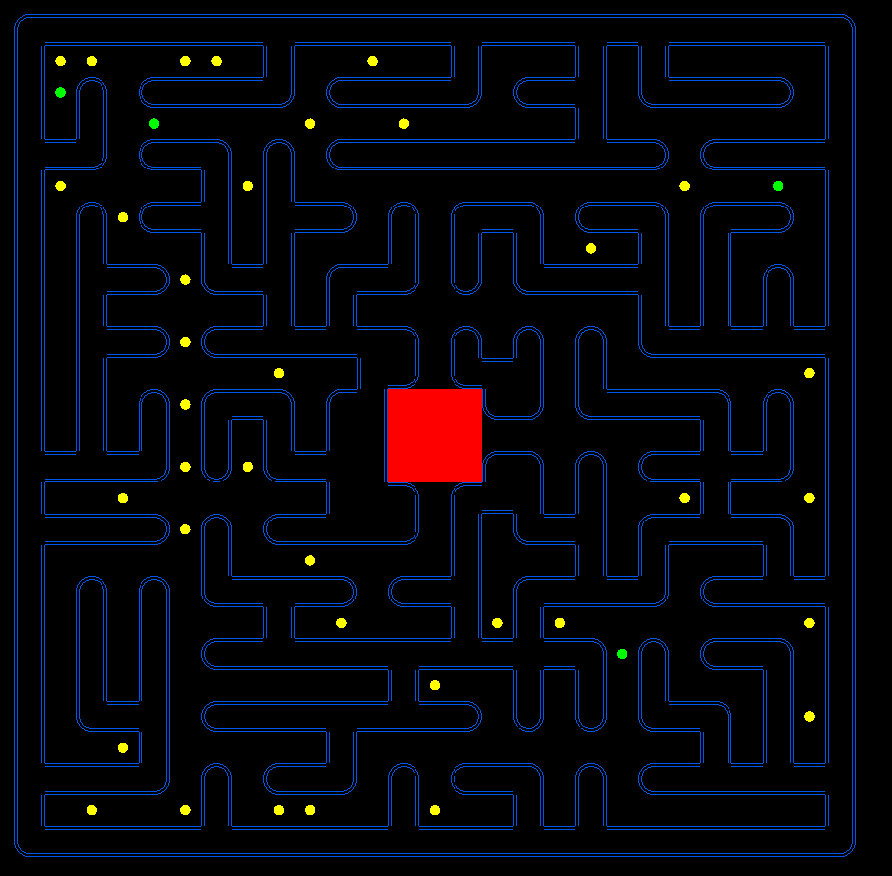
\includegraphics[width=1\textwidth]{images/plateau_42_2.png}
    \caption{Plateau apès génération de la hut}
\end{figure}

L’algorithme de Prim produisant un arbre sans cycles, des ouvertures supplémentaires sont ajoutées de manière aléatoire afin d'ajouter des chemins.
Cette étape améliore la poursuite par les fantômes et évite des trajectoires trop prévisibles.

\begin{figure}[H]
    \centering
    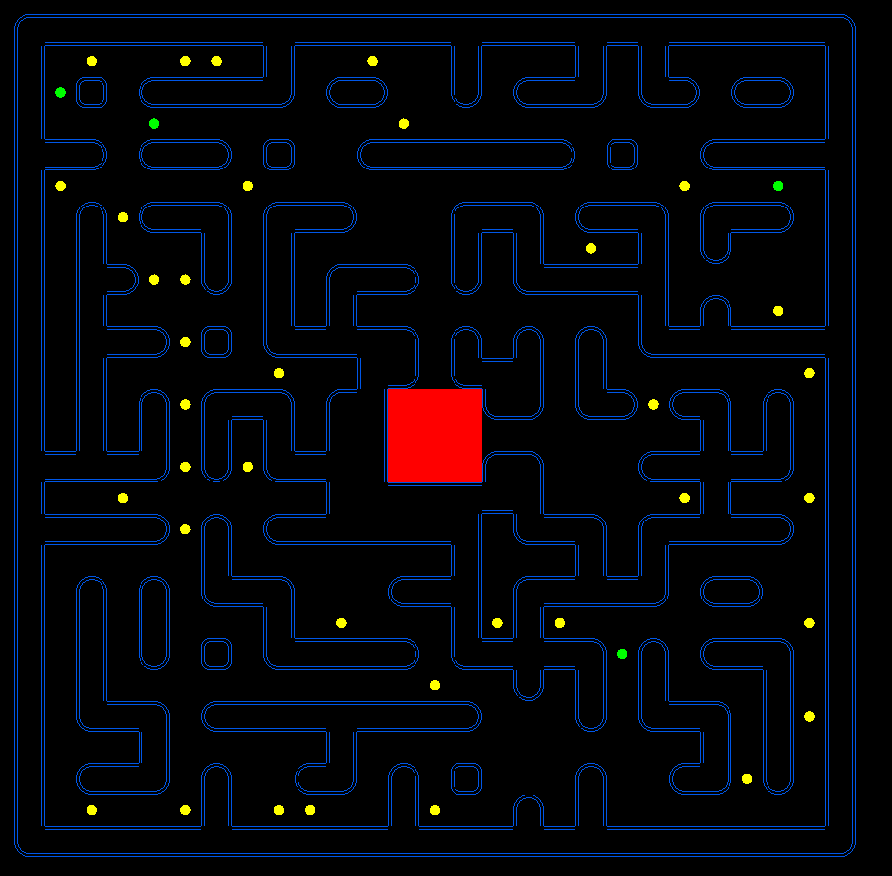
\includegraphics[width=1\textwidth]{images/plateau_42_3.png}
    \caption{Plateau apès ajout de cycles}
\end{figure}

Enfin, certains culs-de-sac sont supprimés en identifiant les cases ne possédant qu’un unique voisin accessible. 
La suppression partielle de ces impasses améliore la fluidité des déplacements et limite les situations punitives.

Des portails latéraux sont également intégrés sur les bords du plateau, ce qui permet à une entité de réapparaître du côté opposé. 

\begin{figure}[H]
    \centering
    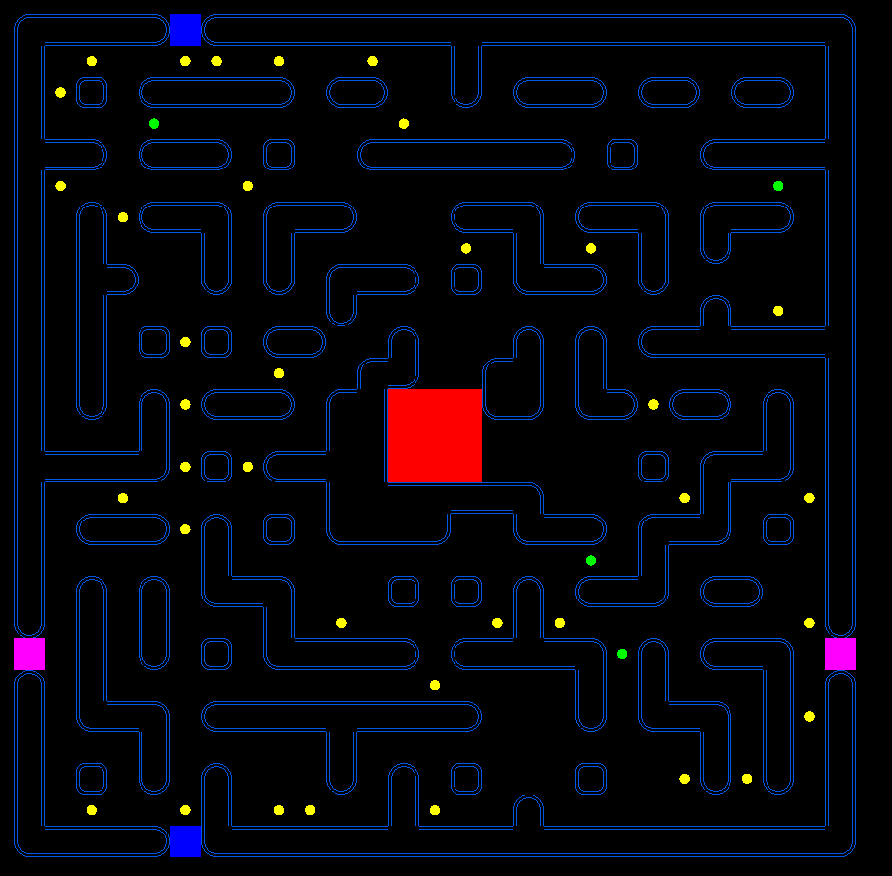
\includegraphics[width=1\textwidth]{images/plateau_42_4.png}
    \caption{Plateau apès suppression des culs-de-sac et ajout des portails}
\end{figure}

Le plateau est une structure centrale du système : il sert de support aux collisions, au placement des pac-gommes, ainsi qu’aux algorithmes de poursuite des fantômes. 
La génération procédurale contribue à la rejouabilité et à la diversité stratégique des parties.

\subsubsection{Intelligence artificielle des fantômes}

L’intelligence artificielle des fantômes repose sur une architecture hybride qui mélange pathfinding classique, système d’influence local et prise de décision hiérarchique. 
L’objectif n’est pas uniquement de poursuivre efficacement Pac-Man, mais de produire une intelligences artificielle adaptable et collective.

\paragraph{Architecture décisionnelle hiérarchique}

À chaque tick serveur, chaque  non joueur évalue sa situation selon un ordre de priorité.

Lorsque Pac-Man est en mode chasseur, la priorité absolue devient la fuite stratégique vers la hut. 
Le plus court chemin est alors calculé à l’aide d’un algorithme de Breadth First Search (BFS), garantissant une trajectoire optimale dans un graphe non pondéré.
Ce choix permet la compatibilité avec les labyrinthes générés procéduralement.

En situation normale, si Pac-Man est détecté dans un rayon de vision défini, le fantôme active un mode de poursuite. 
Un BFS à profondeur limitée est exécuté afin de simuler une perception réduite de l’environnement. 
Cette limitation réduit le coût tout en conservant un comportement crédible et conforme aux regles du jeu.

En l’absence de menace ou de cible visible, le fantôme adopte un comportement autonome fondé sur un système de trace.

\paragraph{Système de trace}

Chaque case du plateau possède un score dynamique défini par :

\[
Score = Attraction - Répulsions
\]

Les traces laissées par Pac-Man génèrent une force attractive, tandis que la présence d’autres fantômes induit des forces répulsives. 
Le fantôme sélectionne localement la case voisine maximisant ce score selon une approche gloutonne.

Ce mécanisme s’inspire des modèles de colonies de fourmis, où l’information est distribuée dans l’environnement. Cela permet de faire une forme d'intelligence collectives peu couteuse.
Ce qui ma donner l'idée d'appliqué ce système et une video sur Youtube : "J'ai codé une simulation de 869 fourmis", de Code Boy%\cite{fourmis}

\paragraph{Comportement émergent}

L’interaction entre attraction vers la cible et répulsion inter-bots produit des comportements collectifs sans coordination explicite. 
Les fantômes tendent naturellement à se disperser, à éviter les regroupements inutiles et à converger progressivement vers Pac-Man en exploitant différentes trajectoires.

\paragraph{Choix algorithmiques}

L’implémentation combine plusieurs techniques complémentaires : 
le BFS pour le calcul de chemins optimaux, une version limitée pour la simulation de vision, une recherche gloutonne locale pour l’exploration autonome.
Un bruit aléatoire est également introduit afin d’éviter les cycles déterministes et les oscillations.

\begin{figure}[H]
    \centering
    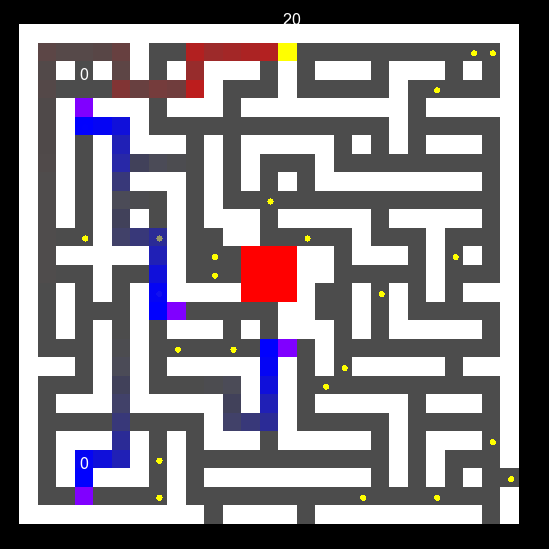
\includegraphics[width=0.8\textwidth]{images/trace.png}
    \caption{Vue des traces}
    \caption*{Rouge pour PacMan et Bleu pour les fantômes}
\end{figure}

\subsubsection{Rooms : gestion des parties}

Afin de supporter plusieurs parties simultanées, le serveur repose sur un système de \textit{rooms}. 
Une room représente une instance autonome de jeu possédant son propre état, ses propres joueurs et son propre cycle d’exécution. 
Cette abstraction permet d’isoler complètement les parties les unes des autres tout en gardant une architecture serveur centralisée.

Chaque room maintient la liste des joueurs connectés, l’attribution des rôles (Pac-Man ou fantômes), les paramètres de la partie ainsi que son état courant (en attente, en cours, terminée). 
Elle encapsule également sa propre boucle de jeu et son plateau, garantissant qu’aucune donnée n’est partagée entre deux parties distinctes.

\paragraph{Création dynamique et attribution des rôles}

Lorsqu’un joueur rejoint le lobby, il est dirigé vers une room existante disposant de places libres. 
Si aucune room n’est disponible, une nouvelle room est créée dynamiquement.
Cette création à la demande permet au serveur d’adapter automatiquement sa structure au nombre de joueurs connectés.

L’attribution des rôles est effectuée au moment du lancement de la partie selon une règle simple : un joueur incarne Pac-Man tandis que les autres deviennent des fantômes. 
Ce mécanisme est géré exclusivement côté serveur afin d’éviter toute incohérence ou manipulation côté client.
En cas de conflit le server informe les clients de la règle non respectée.

\paragraph{Gestion et diffusion de l’état}

Chaque room possède un état centralisé comprenant les positions des joueurs, l’état des pac-gommes et les différents systèmes temporels. 
À chaque tick, cet état est mis à jour puis diffusé uniquement aux joueurs appartenant à la room concernée.

Ce cloisonnement garantit la cohérence interne de chaque partie et empêche toute interférence. 

\paragraph{Paramétrisation des parties}

Les rooms permettent d’ajuster dynamiquement certains paramètres, tels que la durée maximale d’une partie, le nombre de vies de Pac-Man, ect. 
Cette capacité de configuration facilite les phases de test, l’équilibrage du gameplay et l’organisation de parties avec des règles customisées.

\begin{figure}[H]
    \centering
    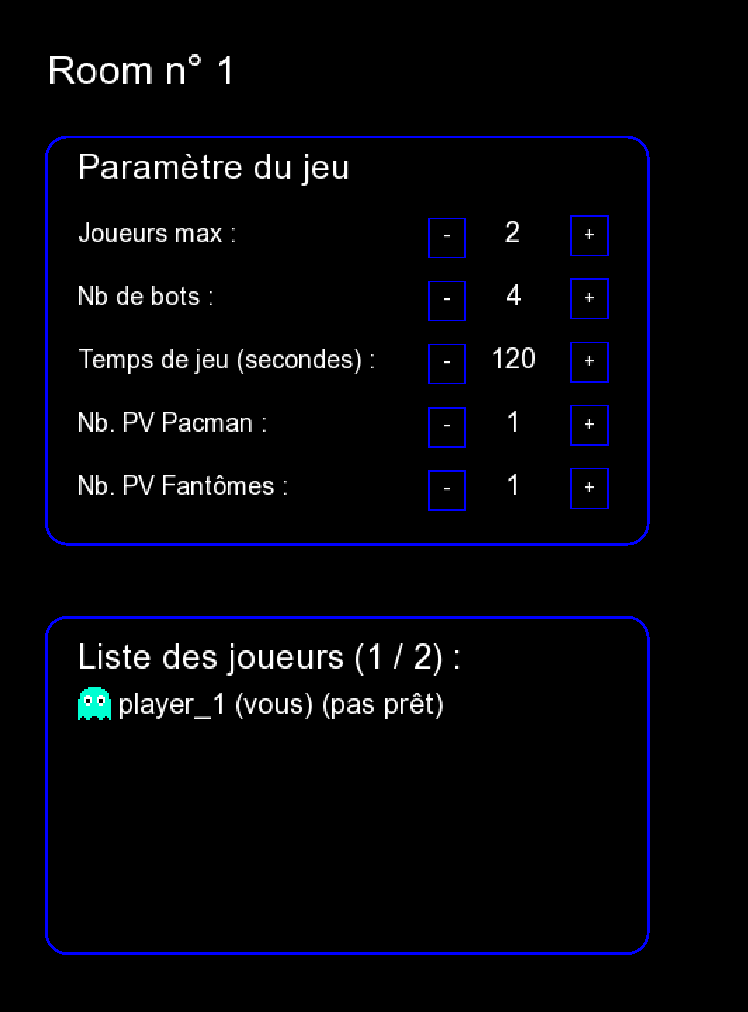
\includegraphics[width=1\textwidth]{images/room.png}
    \caption{Vue de la Room}
\end{figure}



\subsection{Structure du client}

Affichage, gestion des entrées utilisateur,
réception et traitement des messages réseau.

\subsection{Protocoles et échanges réseau}

Description des trames, types de messages,
gestion des événements (connexion, mouvement, fin de partie).


Utilisation de \href{https://gamedevframework.github.io/v1.2.0/classgf_1_1_tcp_socket.html}{gf::TCPSocket} et \href{https://gamedevframework.github.io/v1.2.0/classgf_1_1_tcp_listener.html}{gf::TcpListener}, permettant de faire une tramsmission de données fiable avec le protocol TCP
Socket de connnexion + communication coté serveur, communication uniquement pour le client
Un thread coté client et serveur pour empiler les packet reçu, puis dépilement dans la boucle de jeu pour être traité

Structures de données à la fois utilisé par le serveur et le client (BoardCommonn, PlayerData, RoomSettings, etc...), pas transmit tel quel mais utilisé par les strucutes de com
Exemple illustré avec PlayerData

Structures de communication, contenant parfois ces strucutes communes. gf::Id, pour pouvoir les identifier lors de la déserialisation.
Exemple avec ServerListRoomPlayers

Surchage de l'opétaeur | avec la classe Archive pour les 2 types de structures, nécessaire pour la sérialisation/déserialisation
Exemple illustré avec PlayerData et ServerListRoomPlayers

Sérialisation/Désérialisation avec gf::Packet.is() et gf::Packet.as().
Exemple illustré avec ServerListRoomPlayers

Pour chaque modification on retransmet toutes les données


%\subsection{L'application}

%\subsection{La gestion des tickets}
\newpage


\section{Bilan et perspectives}

\subsection{Compétences acquises}

La réalisation de ce projet nous a permis de mobiliser et d’approfondir plusieurs compétences acquises au cours de notre formation.

Sur le plan technique, nous avons développé des compétences en programmation réseau, notamment dans la conception d’une architecture client-serveur autoritaire, la gestion des communications et la synchronisation d’un système en temps réel.

Le projet a également renforcé nos compétences en architecture logicielle. La transformation d’un prototype vers une structure plus complexes (Server, Lobby, Room, Game) nous a confrontés à des enjeux de séparation des responsabilités, de maintenabilité et d’évolutivité du code. Cette phase de conception a nécessité une réflexion approfondie sur l’organisation des composants et leurs interactions.

Enfin, le travail de conception globale du système, la génération procédurale du plateau, l'implémentation d’une intelligence artificielle, la définition des règles de synchronisation, nous a permis de développer une approche méthodique dans l’analyse des besoins, la modélisation et la résolution de problèmes complexes.

\subsection{Résultat final}

Le projet aboutit à un jeu multijoueur fonctionnel capable de gérer plusieurs connexions simultanées. Les principales fonctionnalités prévues ont été implémentées : gestion des lobbies et des parties, synchronisation en temps réel des joueurs, génération procédurale du labyrinthe, ainsi qu’un système d’intelligence artificielle pour les entités ennemies.

La cohérence du jeu est assurée par les mise à jour périodique côté serveur, ce qui garantit que les états partagés aux clients sont bien valide. Les collision, le déplacement et
les interactions ont été validés et intégrés de manière stable.

\subsection{Améliorations possibles}

Plusieurs axes d’évolution peuvent être envisagés pour enrichir le gameplay et la rejouabilité.

Tous d'abord, introduire des capacités spécifiques aux rôles, telles que : vitesse, invisibilité, téléportation, traversée de murs, invulnérabilité, ou effets sur les ennemis (paralysie, aveuglement, localisation). Ces pouvoirs permettraient des stratégies variées et des interactions plus riches entre joueurs.

Le labyrinthe pourrait inclure plusieurs étages, des salles secrètes, des passages modifiables en cours de partie ou des portails supplémentaires. Ces évolutions augmenteraient la complexité et la diversité des parties.

De plus, Pac-Man pourrait accomplir des missions ou tâches déclenchant des alertes pour les fantômes. Des rôles secrets (traître parmi les fantômes, classe spéciale) pourraient introduire des mécanismes de coopération ou de compétition inattendus.


% Page de conclusion 
\newpage


\section*{Conclusion}
\addcontentsline{toc}{section}{Conclusion}

Ce projet a permis de mettre en pratique les connaissances acquises durant notre formation, notamment en développement réseau, de la programmation multithread et de la conception logicielle et objet.

La création d’un jeu multijoueur inspiré de Pac-Man a nous a permis d’explorer des problématiques telles que la synchronisation des clients, la gestion de plusieurs parties simultanées et la programmation d’une intelligence artificielle pour des entités ennemies.

L’architecture choisi a posé une base solide pour d’éventuelles extensions, comme l’introduction de pouvoirs spéciaux, de rôles secrets ou de labyrinthes multi-étages.

Ainsi, ce projet constitue à la fois un aboutissement des compétences acquises et un terrain d’expérimentation pour de futures évolutions, offrant de nombreuses perspectives d’amélioration et d’enrichissement du gameplay.



% Page de conclusion 
\newpage

\section*{Sitographie}
\addcontentsline{toc}{section}{Sitographie} % Ajout de la sitographie sur la table des matières sans ètre numéroté

\begin{thebibliography}{9}

\bibitem{gf}
Gamedev Framework (gf) 1.2.0,
\url{https://gamedevframework.github.io/v1.2.0/},
consulté le 26 février 2026.

\bibitem{fourmis}
Youtube,
J'ai codé une simulation de 869 fourmis,
de Code Boy,
\url{https://youtu.be/M9ydYnN9_uc?si=7sbFe6XdOyjvBXNl},
consulté le 26 février 2026.



\end{thebibliography}

% Page de résumé
\newpage
\begin{center}
    \vspace*{\fill} % Espace vertical
    \subsection*{Résumé}
    \addcontentsline
    {toc}{section}{Résumé}
    \begin{justify}

        Le projet de la Licence 3 Informatique a été pour nous l’occasion de concevoir et développer un jeu multijoueur inspiré de Pac-Man, en mettant l’accent sur les problématiques de synchronisation réseau, de génération procédurale et d’intelligence artificielle.

        L’objectif principal a été de concevoir une architecture client-serveur autoritaire capable de gérer plusieurs connexions simultanées tout en garantissant la cohérence globale du jeu. Le serveur a été structuré de manière modulaire afin de séparer la gestion réseau, l’organisation des parties et la logique métier.

        Le projet intègre également une génération procédurale de labyrinthe basée sur un algorithme de type Prim adapté aux contraintes du gameplay. L’intelligence artificielle des entités ennemies repose sur une approche hybride combinant recherche de chemin et mécanismes inspiré des fourmis.

        Le développement a été réalisé principalement en C++ avec le Framework Gamedev ainsi que l’utilisation d’outils de gestion de version et de suivi de projet afin d’assurer une organisation structurée du travail.

    \end{justify}
    \vspace*{\fill} % Espace vertical

    \subsection*{Mots-clés}
    \addcontentsline
    {toc}{section}{Mots-Clés}
    \begin{center}
     C++ - PacMan - Gamedev Framework - Réseau - IA
    \end{center}
    \vspace*{\fill} % Espace vertical

    \subsection*{Abstract}
    \addcontentsline
    {toc}{section}{Abstract}
    \begin{justify}
The third-year Computer Science project provided us with the opportunity to design and develop a multiplayer game inspired by Pac-Man, with a particular focus on network synchronization, procedural generation, and artificial intelligence.

The main objective was to design an authoritative client-server architecture capable of handling multiple simultaneous connections while ensuring the overall consistency of the game state. The server was structured in a modular way in order to separate network management, game session organization, and core game logic.

The project also integrates procedural maze generation based on a Prim-like algorithm adapted to gameplay constraints. The artificial intelligence of enemy entities relies on a hybrid approach combining pathfinding techniques and mechanisms inspired by ant colony behavior.

The development was carried out primarily in C++ using the Gamedev framework, along with version control and project management tools to ensure a structured and organized workflow.
    \end{justify}
    \vspace*{\fill} % Espace vertical

    \subsection*{Key-Words}
    \addcontentsline
    {toc}{section}{Key-Words}
    \begin{center}
    C++ - PacMan - Gamedev Framework - Network - AI
    \end{center}
    \vspace*{\fill} % Espace vertical
    
    
\end{center}

\end{document}